\appendix
	\part*{Annexes}	
	\addcontentsline{toc}{part}{Annexes}
	\setcounter{chapter}{0}

\chapter{\label{annexe_index_schoepflin}Les index de la Renaissance, termes contrôlés et classification alphabétique (les index de l'\textit{Alsatia Illustrata} de \nP{Jean-Daniel}{Schoepflin})}
\titreEntete{Annexe \thechapter}

\begin{figure}[!h]
	\centering
	\begin{minipage}[c]{.46\linewidth}
		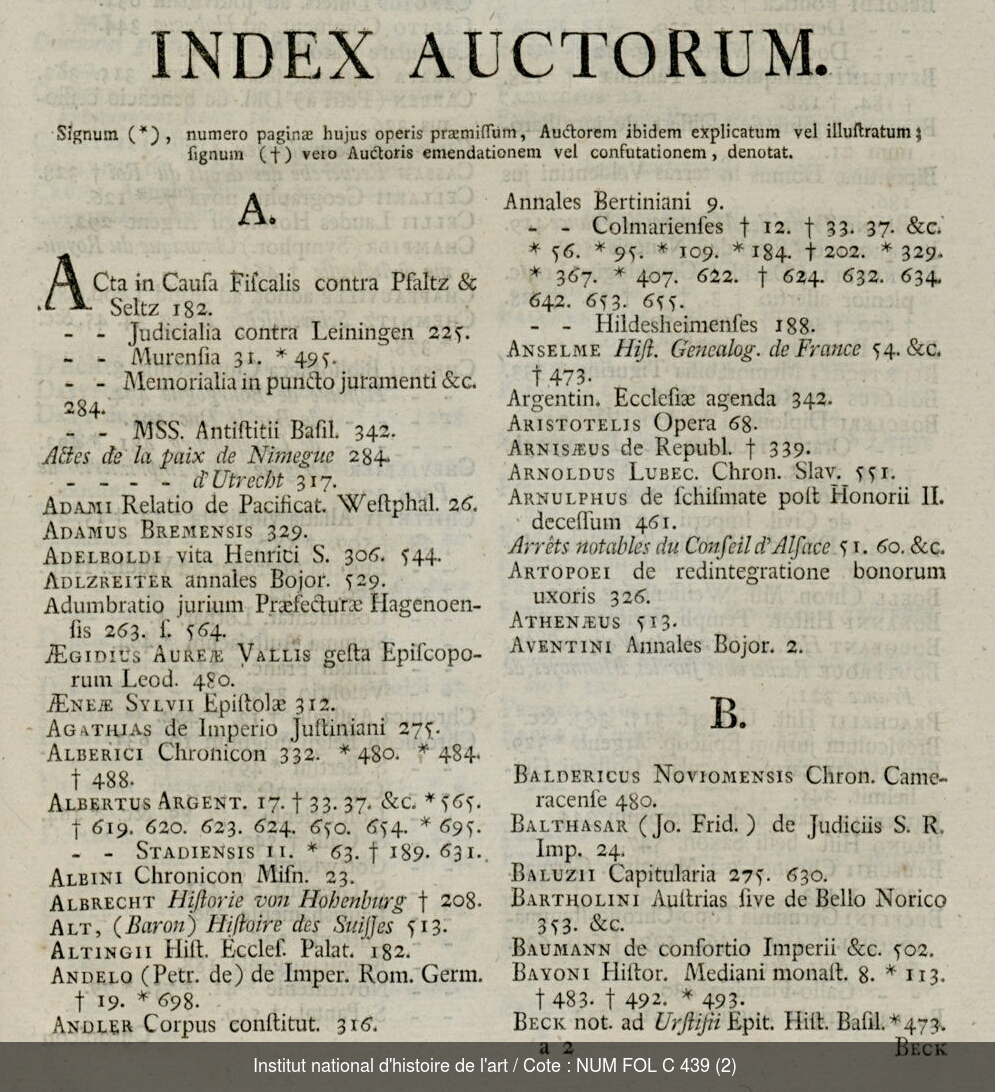
\includegraphics[width=6cm]{images/index_auctorum_alsatia.jpg}
		\caption{Index auctorum}
	\end{minipage} \hfill
	\begin{minipage}[c]{.46\linewidth}
		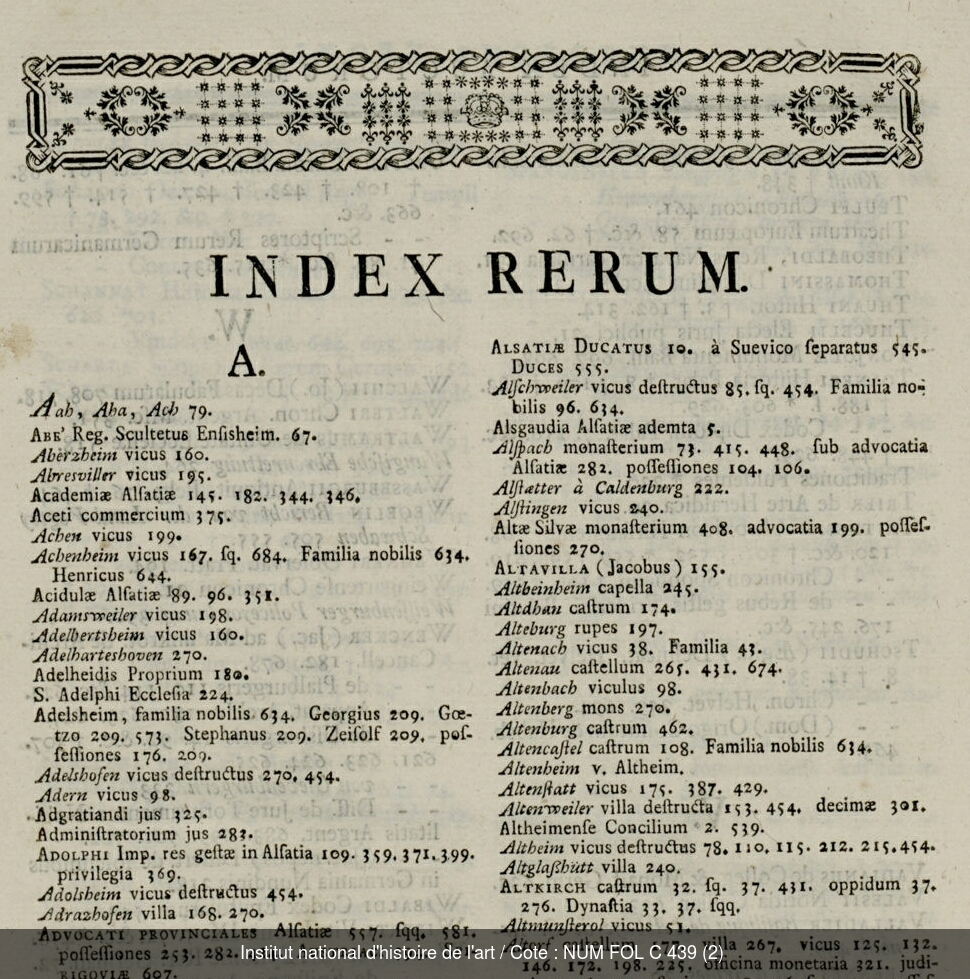
\includegraphics[width=6cm]{images/index_rerum_alsatia.jpg}
		\caption{Index rerum}
	\end{minipage} 
	\medskip
	Extraits des deux index de l'œuvre de \nP{Jean-Daniel}{Schoepflin} [Source: \url{http://bibliotheque-numerique.inha.fr/idurl/1/12532}, p.804 et 813]
\end{figure}

\chapter{\label{annexe_types_interop}Les différents types d'interopérabilité}
\titreEntete{Annexe \thechapter}

\begin{figure}[!h]
	\centering
	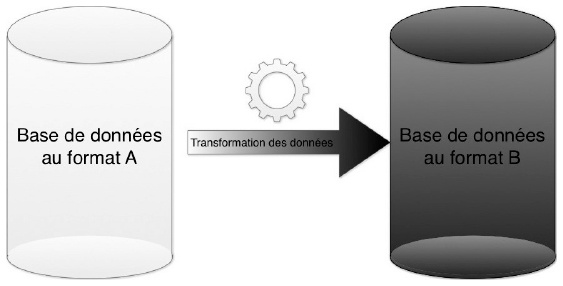
\includegraphics[width=12cm]{images/interop_conversion_copie.jpeg}
	\medskip
	\caption[L'interopérabilité par conversion et copie]{L'interopérabilité par conversion et copie [Source: \cite{bermes_2_2013}]}
\end{figure}

\begin{figure}[!h]
	\centering
	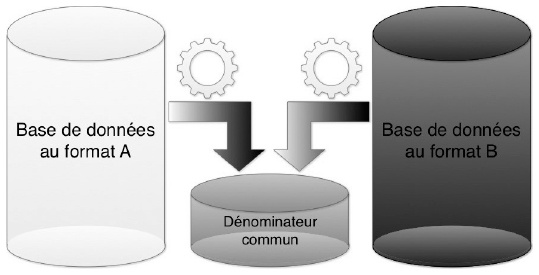
\includegraphics[width=12cm]{images/interop_denom_commun.jpeg}
	\medskip
	\caption[L'interopérabilité par le plus petit dénominateur commun]{L'interopérabilité par le plus petit dénominateur commun [Source: \cite{bermes_2_2013}]}
\end{figure}

\begin{figure}[!h]
\centering
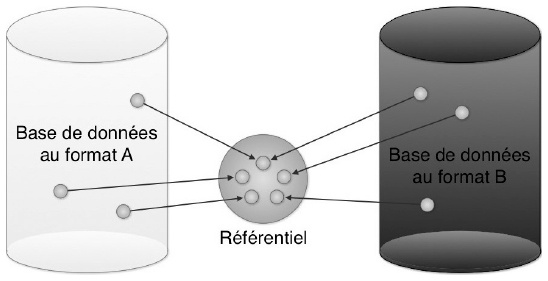
\includegraphics[width=12cm]{images/interop_hub_spoke.jpeg}
\medskip
\caption[L'interopérabilité de le roue et de l'essieu]{L'interopérabilité de la roue et de l'essieu [Source: \cite{bermes_2_2013}]}
\label{hub_spoke}
\end{figure}

\begin{figure}[!h]
	\centering
	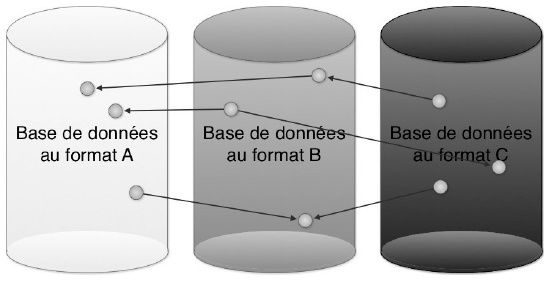
\includegraphics[width=12cm]{images/interop_follow_nose.jpeg}
	\medskip
	\caption[L'interopérabilité par parcours de liens]{L'interopérabilité par parcours de liens [Source: \cite{bermes_2_2013}]}
	\label{interop_follow_nose}
\end{figure}

\chapter{\label{annexe_type_donnees_axel}Les types de données présents dans les bases de données de l'\ac{ina} et leur rôle}
\titreEntete{Annexe \thechapter}

\begin{figure}[!h]
	\centering
	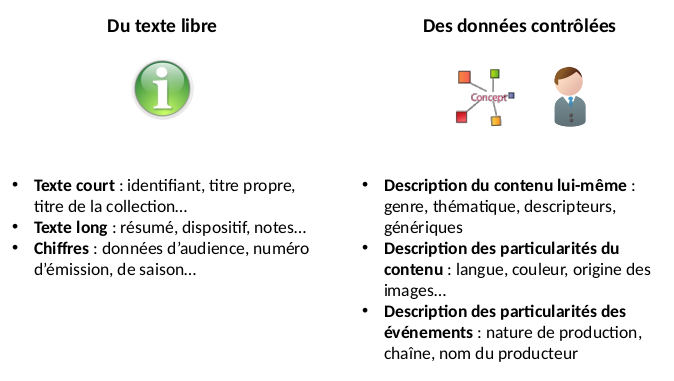
\includegraphics[width=15cm]{images/type_donnees_axel.png}
	\medskip
	\caption[Les types de données présents dans les bases de données de l'\ac{ina}]{Les types de données présents dans les bases de données de l'\ac{ina} [Source: \cite[p.6]{roche-diore_atelier_2020}]}
	\label{type_donnees_axel}
\end{figure}

\chapter{\label{annexe_bdd_ina}Les bases de données de la \ac{ddcol} de l'\ac{ina}}
\titreEntete{Annexe \thechapter}

\begin{figure}[!h]
	\centering
	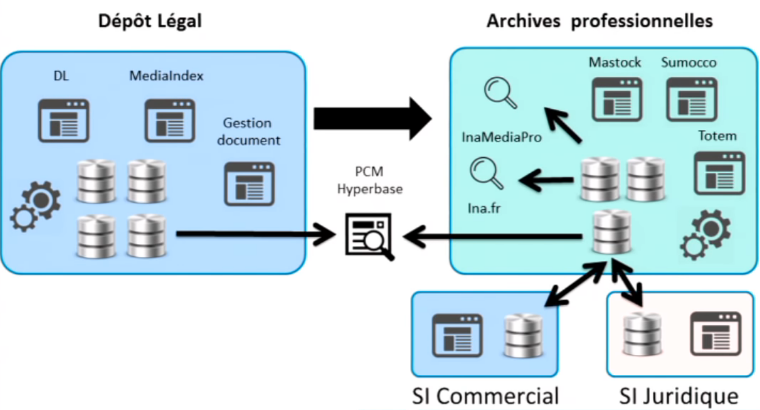
\includegraphics[width=15cm]{images/bases_ddcol.png}
	\medskip
	\caption[Les bases de données de la \ac{ddcol} de l'\ac{ina}]{Les bases de données de la \ac{ddcol} de l'\ac{ina} [Source: \cite{poupeau_rassembler_2019}]}
	\label{bdd_ddcol_ina}
\end{figure}


\chapter{\label{annexe_thesaurus}Le thésaurus de noms communs de l'\ac{ina}}
\titreEntete{Annexe \thechapter}

\begin{figure}[!h]
	\centering
	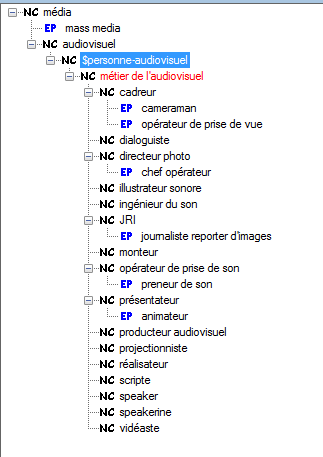
\includegraphics[width=7cm]{images/cadreur_hierarchie.png}
	\medskip
	\caption[Extrait du thésaurus de noms communs de l'\ac{ina}]{Extrait du thésaurus de noms communs de l'\ac{ina} autour du terme \og Cadreur\fg{}}
	\label{thesaurus_cadreur}
\end{figure}

\chapter{\label{annexe_alignement_journaliste}Aligner les fonctions de \og Journaliste\fg{} des notes qualité avec le thésaurus des noms communs de l'\ac{ina}}
\titreEntete{Annexe \thechapter}

\begin{figure}[!h]
	\centering
	\csvautotabular[separator=semicolon]{images/alignement_journaliste.csv}
	\caption{Résultat de l'alignement des journalistes avec le thésaurus des noms communs}
	\label{alignement_journaliste}
\end{figure}

\chapter{\label{annexe_dl_captation}Les captations directes réalisées par l'\ac{ina} au titre du dépôt légal}
\titreEntete{Annexe \thechapter}

\begin{figure}[!h]
	\centering
	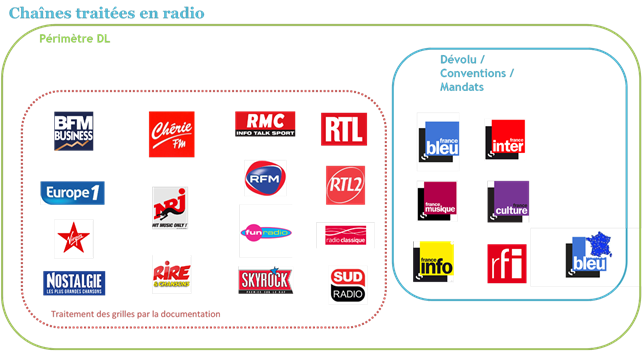
\includegraphics[width=16cm]{images/dl_radio.png}
	\caption[Stations de radio captées au titre du dépôt légal]{Stations de radio captées au titre du dépôt légal [Source: Communication électronique  de l'entreprise \og La collecte et le catalogage\fg{} du 26 mai 2020]}
	\label{dl_radio}
\end{figure}

\begin{figure}[!h]
	\centering
	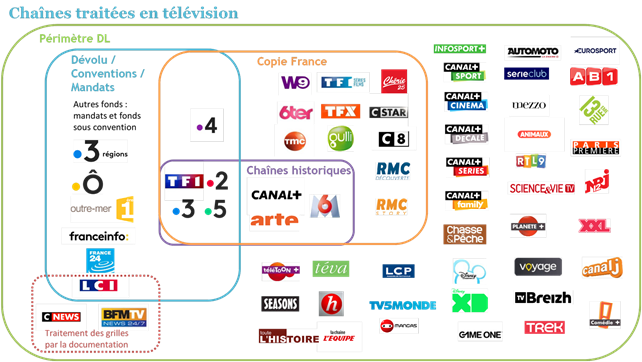
\includegraphics[width=16cm]{images/dl_tv.png}
	\caption[Chaînes de télévision captées au titre du dépôt légal]{Chaînes de télévision captées au titre du dépôt légal [Source: Communication électronique  de l'entreprise \og La collecte et le catalogage\fg{} du 26 mai 2020]}
	\label{dl_tv}
\end{figure}

\chapter{\label{annexe_fournisseurs_exterieurs}Les fournisseurs externes de données de l'\ac{ina}}
\titreEntete{Annexe \thechapter}

\begin{figure}[!h]
	\centering
	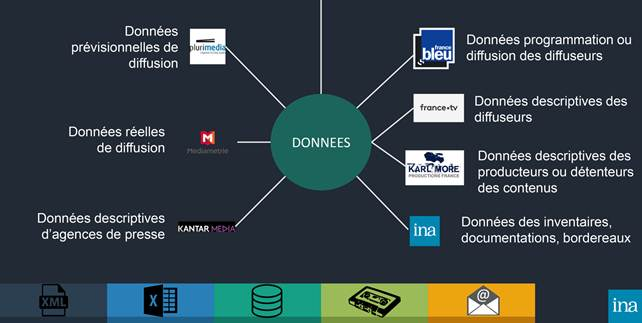
\includegraphics[width=16cm]{images/enrichissement_dl.jpg}
	\caption[Les fournisseurs extérieurs de données de l'\ac{ina}]{Les fournisseurs extérieurs de données de l'\ac{ina} [Source: Communication électronique  de l'entreprise \og La collecte et le catalogage\fg{} du 26 mai 2020]}
	\label{enrichissement_dl}
\end{figure}

\begin{table}
	\centering
	\begin{tabularx}{16cm}{|X|X|X|X|}
		\hline
		 \begin{center}ID INA\end{center}&\begin{center}CHAINE CODE\end{center}&\begin{center}DOC TITRE COLLECTION\end{center}&\begin{center}DOC TITRE PROPRE\end{center}  \tabularnewline \hline
		 \begin{center}550274 010 3\end{center}&\begin{center}N12\end{center}&\begin{center}The Big Bang Theory\end{center}&\begin{center}La phobie de Sheldon\end{center}  \tabularnewline \hline
		 \begin{center}DOC DATE\end{center}&\begin{center}DOC HEURE DEBUT\end{center}&\begin{center}DOC HEURE FIN\end{center}&\begin{center}DOC NUMERO EPISODE\end{center}  \tabularnewline \hline
		 \begin{center}20160312\end{center}&\begin{center}124404\end{center}&\begin{center}130424\end{center}&\begin{center}S5-9\end{center}  \tabularnewline \hline
		 \begin{center}DOC NOMBRE EPISODES\end{center}&\begin{center}DOC DUREE\end{center}&\begin{center}DOC REPERAGE\end{center}&\begin{center}DOC COULEUR\end{center}  \tabularnewline \hline
		 \begin{center}24\end{center}&\begin{center}00202000\end{center}&\begin{center}12440400\end{center}&\begin{center}C\end{center}  \tabularnewline \hline
		 \begin{center}DOC TAUX MA\end{center}&\begin{center}DOC PART DA\end{center}&\begin{center}DOC TAUX MOYEN 15\end{center}&\begin{center}DOC PART MOYEN 15\end{center}  \tabularnewline \hline
		 \begin{center}0.7\end{center}&\begin{center}2.9\end{center}&\begin{center}0.7\end{center}&\begin{center}3\end{center}  \tabularnewline \hline
		 \begin{center}DOC TAUX MOYEN FEMME\end{center}&\begin{center}DOC TAUX MOYEN HOMME\end{center}&\begin{center}DOC DATE DERN MODIF\end{center}&\begin{center}DOC LIEN REDIFFUSION\end{center}  \tabularnewline \hline
		 \begin{center}0.6\end{center}&\begin{center}0.9\end{center}&\begin{center}20171016\end{center}&\begin{center}S:345421.025\end{center}  \tabularnewline \hline
		 \begin{center}DOC DATE CREATION\end{center}&\begin{center}MEDIAMETRIE REF\end{center}&\begin{center}ANNEE PRODUCTION\end{center}&\begin{center}IMEDIA REF\end{center}  \tabularnewline \hline
		 \begin{center}20160315\end{center}&\begin{center}56881\end{center}&\begin{center}2011\end{center}&\begin{center}35858990 \end{center}  \tabularnewline \hline
	\end{tabularx}
\caption[L'apport des données de Médiamétrie dans la description effectuée au \ac{dl}]{L'apport des données de Médiamétrie dans la description effectuée au \ac{dl} [Source: extrait de la base de données DLSAT de l'\ac{ina}]}
\label{sheldon_mediametrie}
\end{table}

\chapter{\label{annexe_lod}La constellation du Linked Open Data}
\titreEntete{Annexe \thechapter}

\begin{figure}[!h]
	\centering
	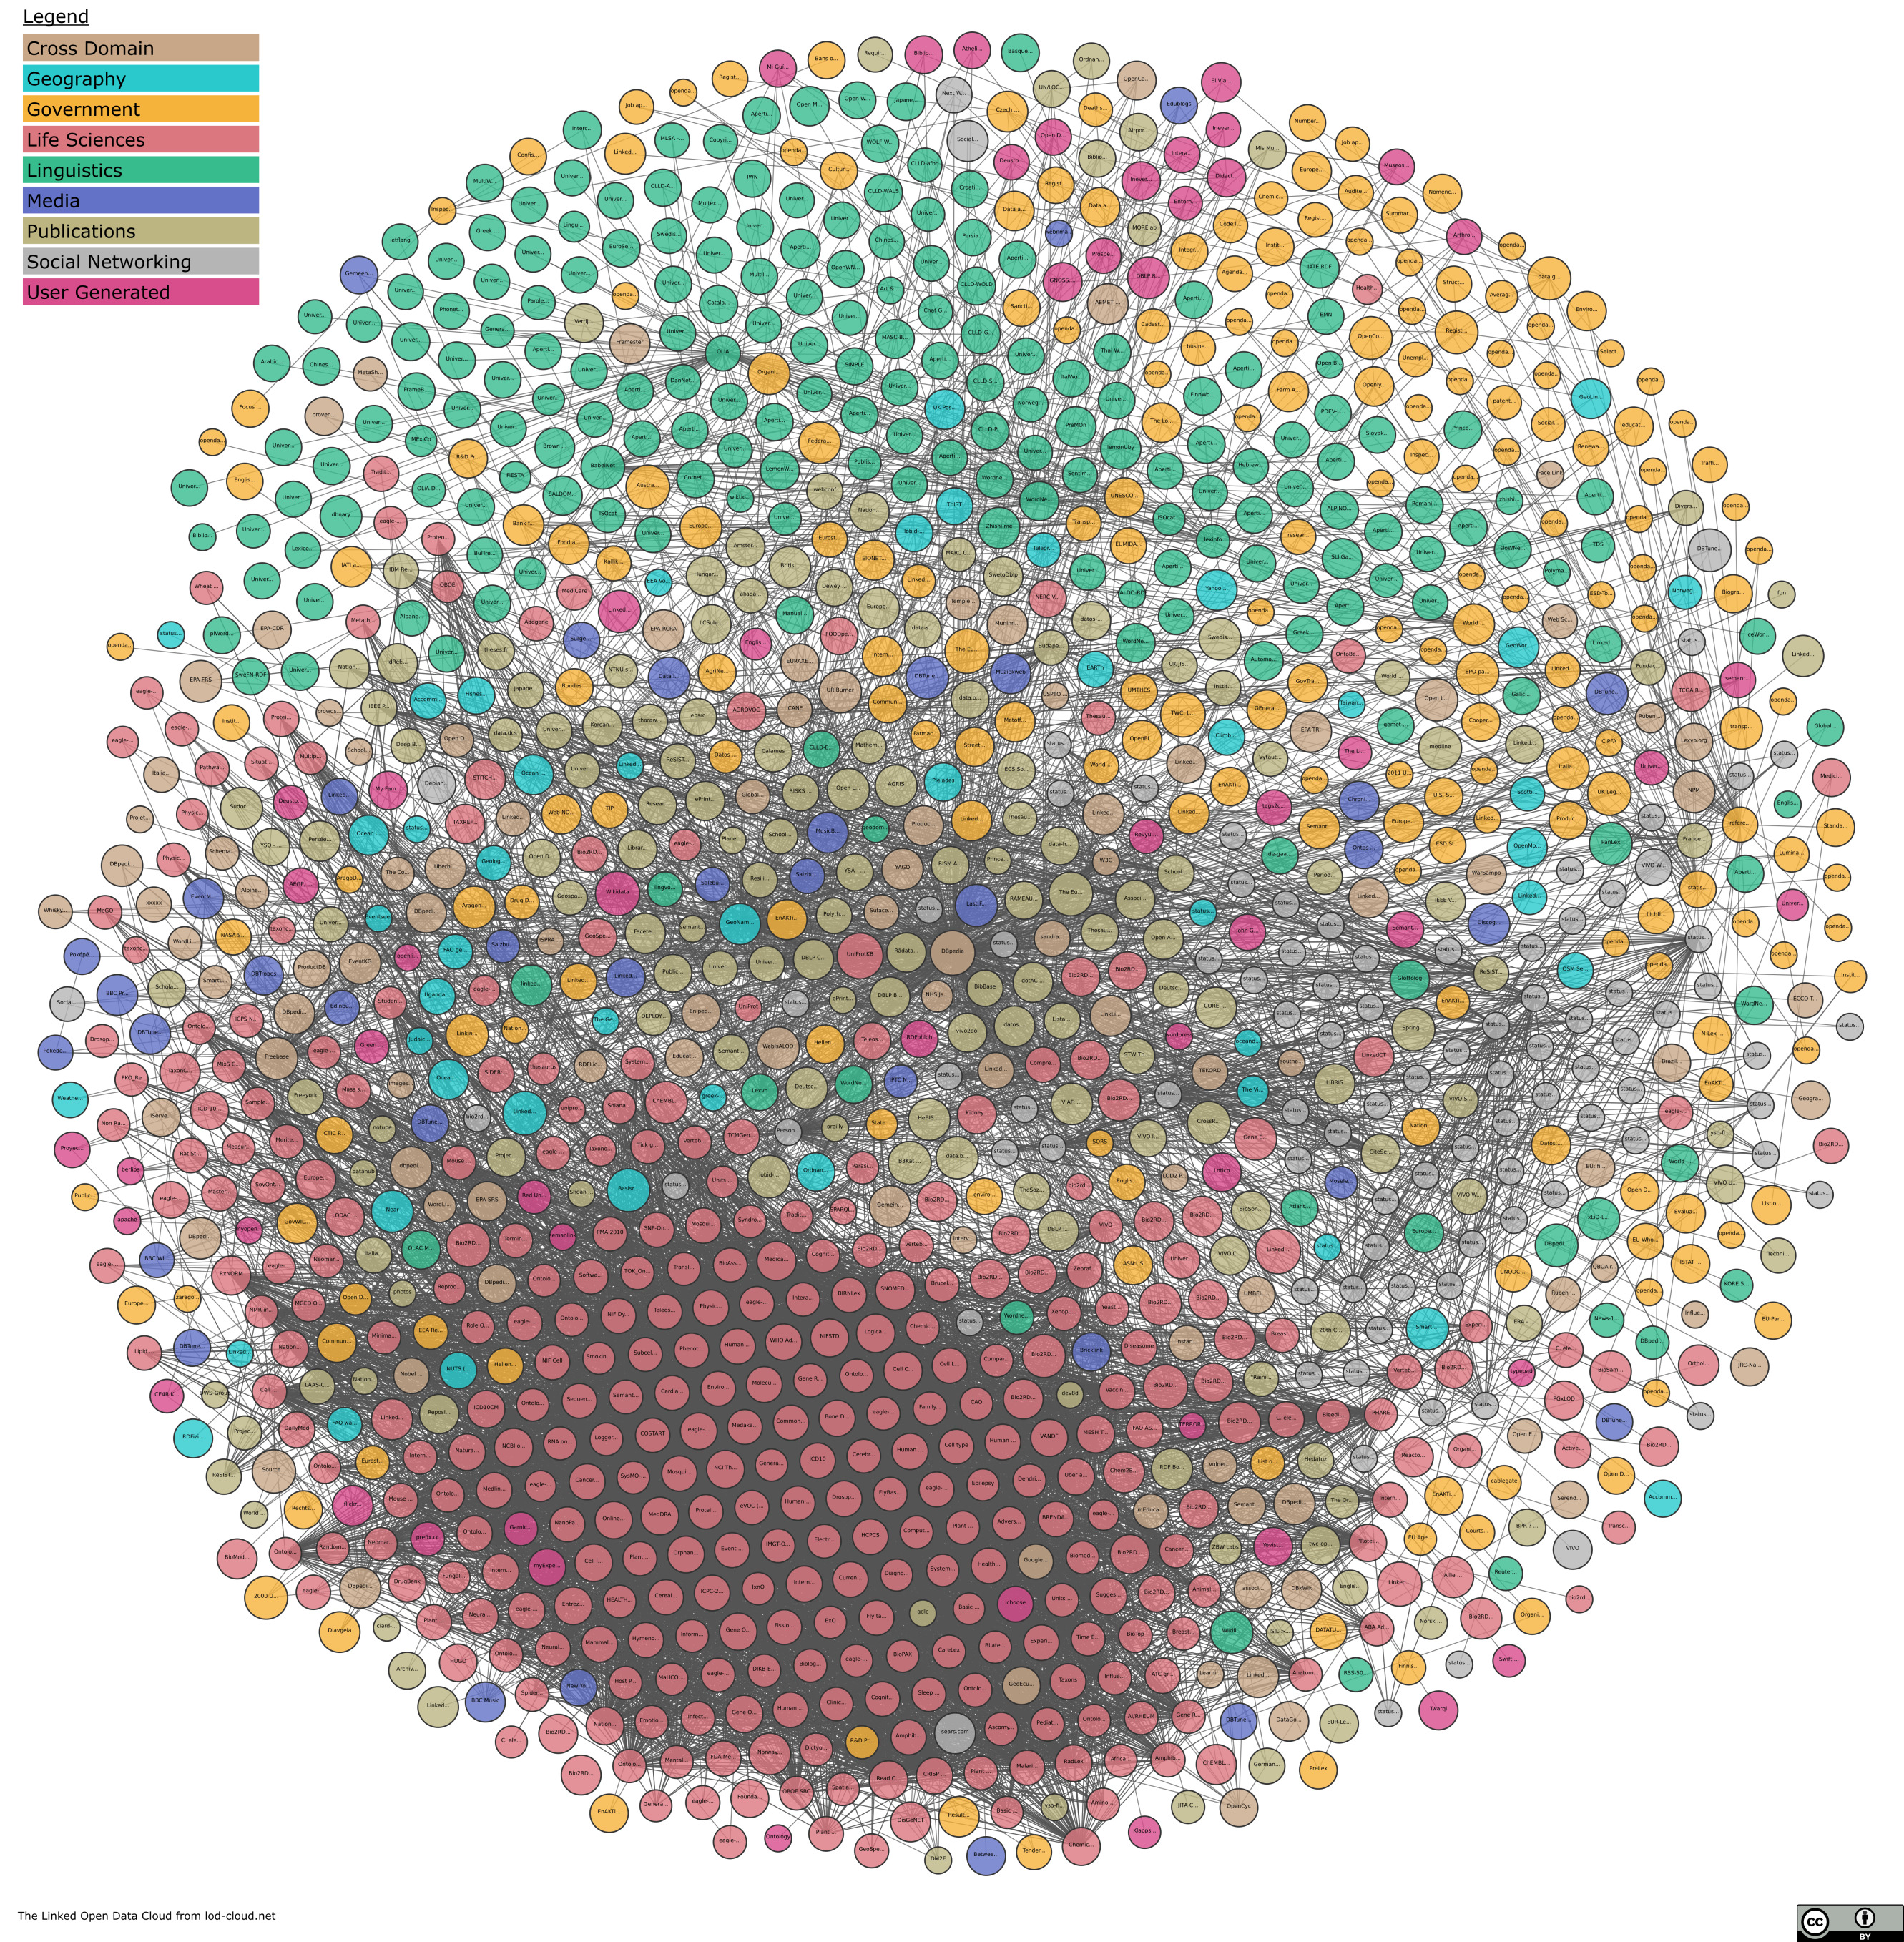
\includegraphics[width=16cm]{images/lod-cloud-sm.jpg}
	\caption[La constellation du Linked Open Data en juillet 2020]{La constellation du Linked Open Data en juillet 2020 [Source: \cite{noauthor_linked_2020}]}
	\label{lod_cloud}
\end{figure}

\chapter{\label{annexe_nvx_modeles}Repenser la place du référentiel}
\titreEntete{Annexe \thechapter}

\begin{figure}[!h]
	\centering
	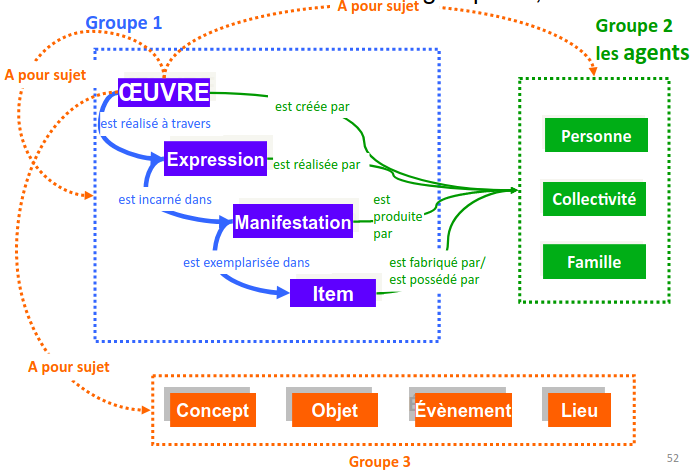
\includegraphics[width=16cm]{images/frbr_slide.png}
	\caption[Le modèle \ac{frbr}]{Le modèle \ac{frbr} [Source: \cite[s.52]{benezet_participer_2015}]}
	\label{frbr}
\end{figure}

\begin{figure}[!h]
	\centering
	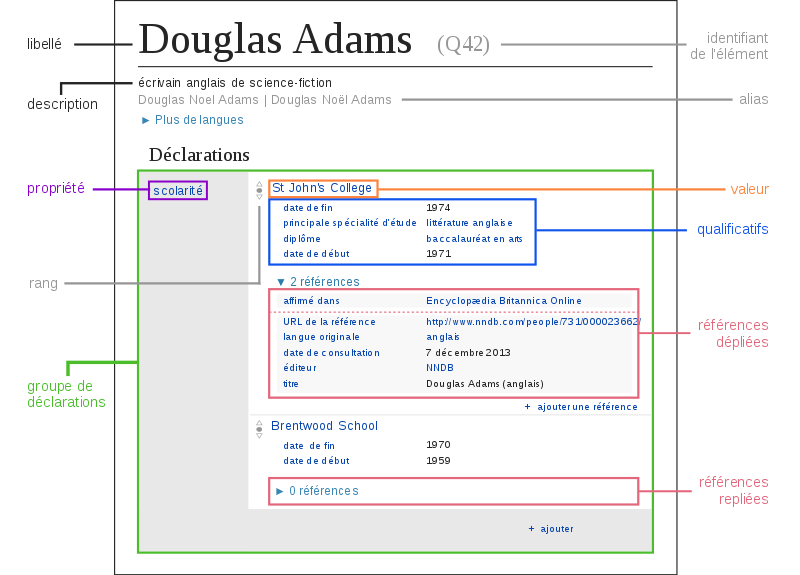
\includegraphics[width=16cm]{images/modele_wikidata.png}
	\caption[Le modèle de données de Wikidata]{Le modèle de données de Wikidata [Source: \href{https://upload.wikimedia.org/wikipedia/commons/thumb/c/ce/Datamodel_in_Wikidata_fr.svg/330px-Datamodel_in_Wikidata_fr.svg.png}{Wikimédia}]}
	\label{wikidata}
\end{figure}

\begin{figure}[!h]
	\centering
	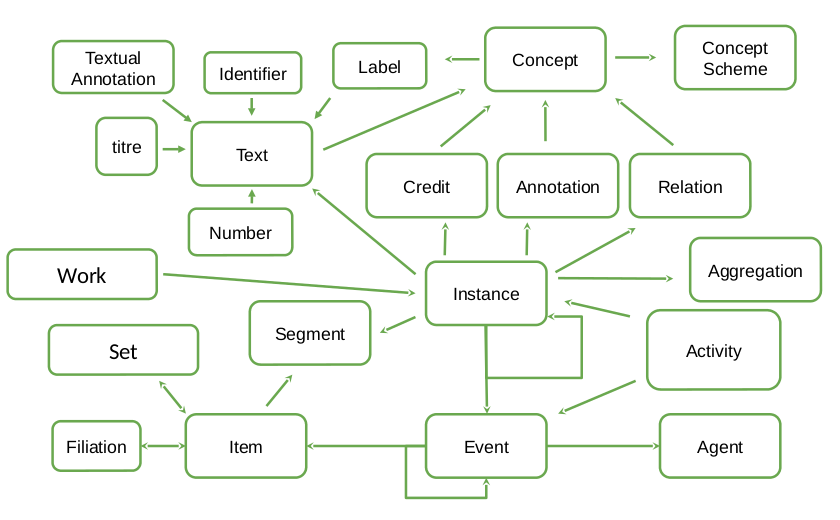
\includegraphics[width=16cm]{images/schema_global_lac.png}
	\caption[Le modèle de données du \ldd à l'\ac{ina}]{Le modèle de données du \ldd à l'\ac{ina} [Source:\cite[d.13]{roche-diore_atelier_2020}}
	\label{modele_ldd}
\end{figure}

\chapter{\label{annexe_lac}Repenser l'infrastructure}
\titreEntete{Annexe \thechapter}

\begin{figure}[!h]
	\centering
	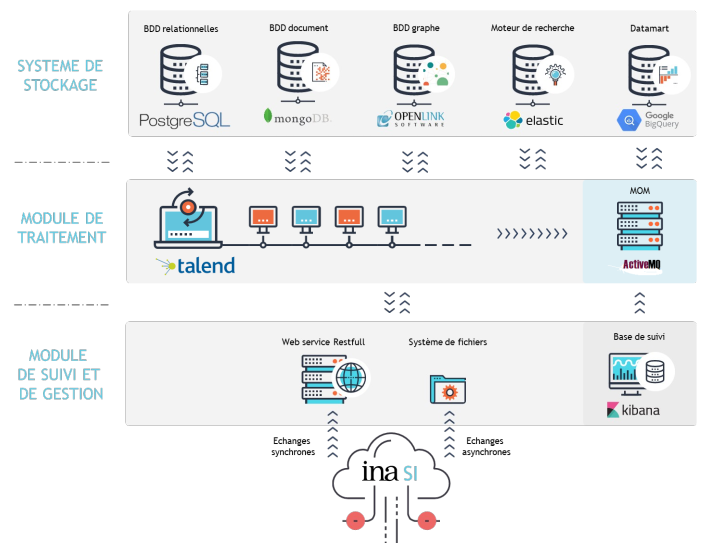
\includegraphics[width=16cm]{images/infrastructure_unique.png}
	\caption[Schéma du \ldd depuis le stockage jusqu'à l'accès aux données]{Schéma du \ldd depuis le stockage jusqu'à l'accès aux données [Source: \cite{poupeau_rassembler_2019}]}
	\label{lac_infra}
\end{figure}

\chapter{\label{annexe_onto}Ontologies de haut et de bas niveaux}
\titreEntete{Annexe \thechapter}

\begin{figure}[!h]
	\centering
	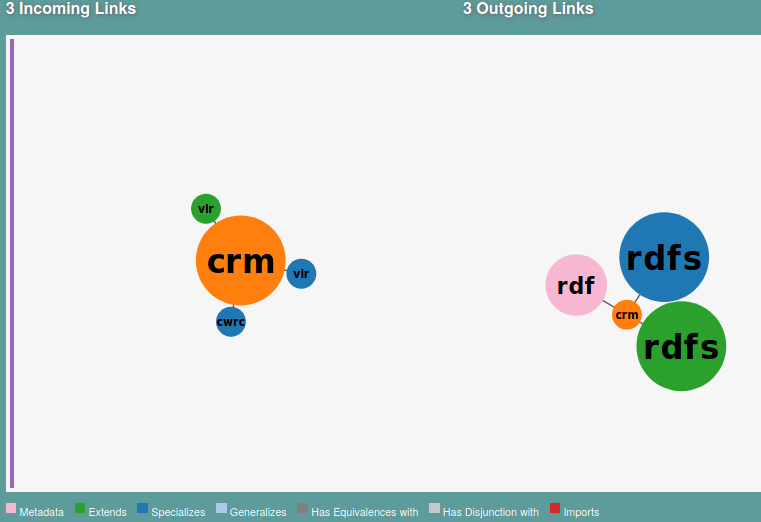
\includegraphics[width=14cm]{images/onto_crm.png}
	\caption[Une ontologie de haut niveau: CIDOC-CRM]{Une ontologie de haut niveau: représentation des ontologies utilisant celle du \ac{cidoccrm}(à gauche) et de celles utilisées par l'ontologie du \ac{cidoccrm}(à droite) [Source: \url{https://lov.linkeddata.es/dataset/lov/vocabs/crm}]}
	\label{onto_crm}
\end{figure}

\begin{figure}[!h]
	\centering
	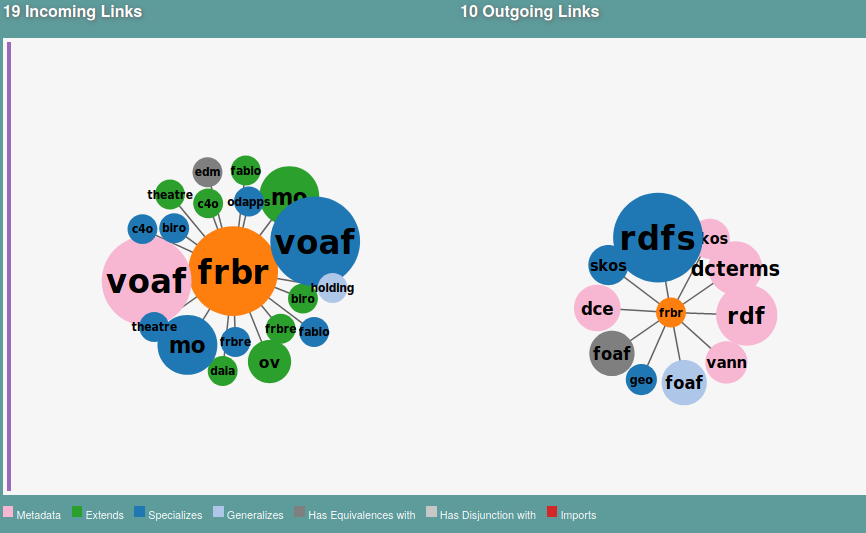
\includegraphics[width=14cm]{images/onto_frbr.png}
	\caption[Une ontologie de domaine: FRBR]{Une ontologie de domaine: représentation des ontologies utilisant celle du \ac{frbr}(à gauche) et de celles utilisées par l'ontologie du \ac{frbr}(à droite) [Source: \url{https://lov.linkeddata.es/dataset/lov/vocabs/frbr}]}
	\label{onto_frbr}
\end{figure}

\begin{figure}[!h]
	\centering
	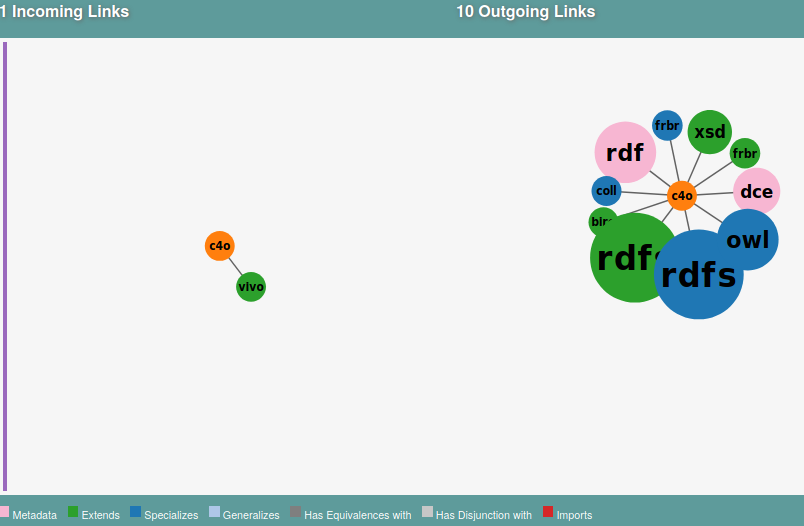
\includegraphics[width=14cm]{images/onto_c4o.png}
	\caption[Une ontologie applicative: C4O]{Une ontologie applicative: représentation des ontologies utilisant C4O (à gauche) et de celles utilisées par l'ontologie C4O(à droite) [Source: \url{https://lov.linkeddata.es/dataset/lov/vocabs/c4o}]}
	\label{onto_c4o}
\end{figure}

\chapter{\label{annexe_laby}Labyrinthes}
\titreEntete{Annexe \thechapter}

\begin{figure}[!h]
	\centering
	\begin{minipage}[c]{.46\linewidth}
		
\includegraphics[width=6cm]{images/laby_knossos.png}
		\caption[Le labyrinthe de Knossos]{Le labyrinthe de Knossos [Source: \cite[ch. 1.5]{eco_arbre_2010}]}
		\label{laby_knossos}
	\end{minipage}
	\begin{minipage}[c]{.46\linewidth}
		
\includegraphics[width=6cm]{images/laby_irrweg.png}
		\caption[Le labyrinthe d'Irrweg]{Le labyrinthe d'Irrweg [Source: \cite[ch. 1.5]{eco_arbre_2010}]}
		\label{laby_irrweg}
\end{minipage}
\end{figure}

\begin{figure}[!h]
	\centering
		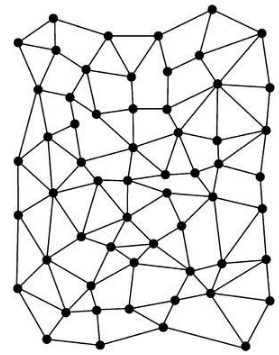
\includegraphics[width=6cm]{images/laby_reseau.png}
		\caption[Le labyrinthe réseau]{Le labyrinthe réseau [Source: \cite[ch. 1.5]{eco_arbre_2010}]}
		\label{laby_reseau}
\end{figure}